\documentclass[10pt,a4paper]{article}

\usepackage[top=1cm,bottom=2cm]{geometry}
\usepackage{graphicx}
\usepackage[backend=bibtex]{biblatex}
\usepackage{hyperref}
\bibliography{report.bib}
\author{Christoffer Jansson \and Alan Khudur \and Dmitrij Lioubartsev \and Michal Staniaszek \and Yavor Trasiev}
\title{DD2425 Robotics and Autonomous Systems Final Report}

\begin{document}
\maketitle
\begin{abstract}
  In this report we describe our hardware and software solutions for the house
  service robot task set in the DD2425 Robotics and Autonomous Systems course.
  The task required the construction of a robot from a limited set of materials,
  and the implementation of a software system using the Robot Operating System
  (ROS)\cite{rosorg} framework. We implemented a control system for motion in
  the maze, including wall following, a vision system to make use of the
  Primesense RGB-D camera, and additional systems for mapping.
\end{abstract}
\section{Task Specification}
The website for the course specifies the task as follows:
\begin{quote}
  \emph{Your robot is the new service robot is someone's house. The new owner has just
  turned on the robot and given it a few minutes to have a look around in the
  new environment. Your robot should take this chance to learn as much as
  possible about the environment so that it can be as good as possible in future
  tasks. It should learn to find its way and it should detect and remember where
  certain objects are.}
\end{quote}
This specification is a description of a real world task that might be performed
by a robot. Since we had only two months to implement the system, the actual
task that had to be performed was somewhat simplified. The ``house'' was
replaced by a maze made of straight pieces of wood, with all of the walls having
either a horizontal or vertical orientation --- there are no diagonal walls. The
robot should detect and remember the location of are various brightly coloured
shapes, seen in Figure~\ref{fig:shapes}.

The task can be broken into two phases, each of which has a distinct purpose. In
the first phase, the robot must explore the environment and learn where objects
are. In the second phase, which is not described explicitly in the
specification, the robot should return to the previously discovered object
locations and ``fetch'' the objects.

Although these tasks would be trivial for any human, for a robot to do them
autonomously is a very demanding task, even in a restricted environment such as
the one we will be operating in. To complete the first phase, we must be able to
move the robot, which requires the implementation of controllers which allow the
robot to move based on demands on angular and linear velocity. A wall following
system is also required, to use the structure of the environment to explore it.
This requires the use of sensors to detect walls to the side and in front of the
robot to prevent collisions, and detect when it is possible for the robot to
turn. A vision system which can detect objects and correctly identify them is
also needed. A map must also be constructed and stored so that the position of
objects can be remembered for use in the second phase. During the second phase,
some sort of path planning is required to move efficiently between the different
objects. The ability to localise within the created map is also necessary in
order for the robot to know the position of objects and walls relative to its
own location. In addition, a way of navigating between specific locations in the
map is required.

To complete the full task, we had to design and build a robot, and write
software for all of these subsystems. The subsequent sections describe our
approach to each problem and how we solved it, including some of the ideas that
we did not use, and the reasons for that, as well as some analysis of the
performance of each of the subsystems.

\begin{figure}
  \centering
  \includegraphics[width=\linewidth]{images/objects.jpg}
  \caption{Objects to be detected within the maze.}
  \label{fig:shapes}
\end{figure}
\section{Hardware}
\begin{figure}
  \centering
  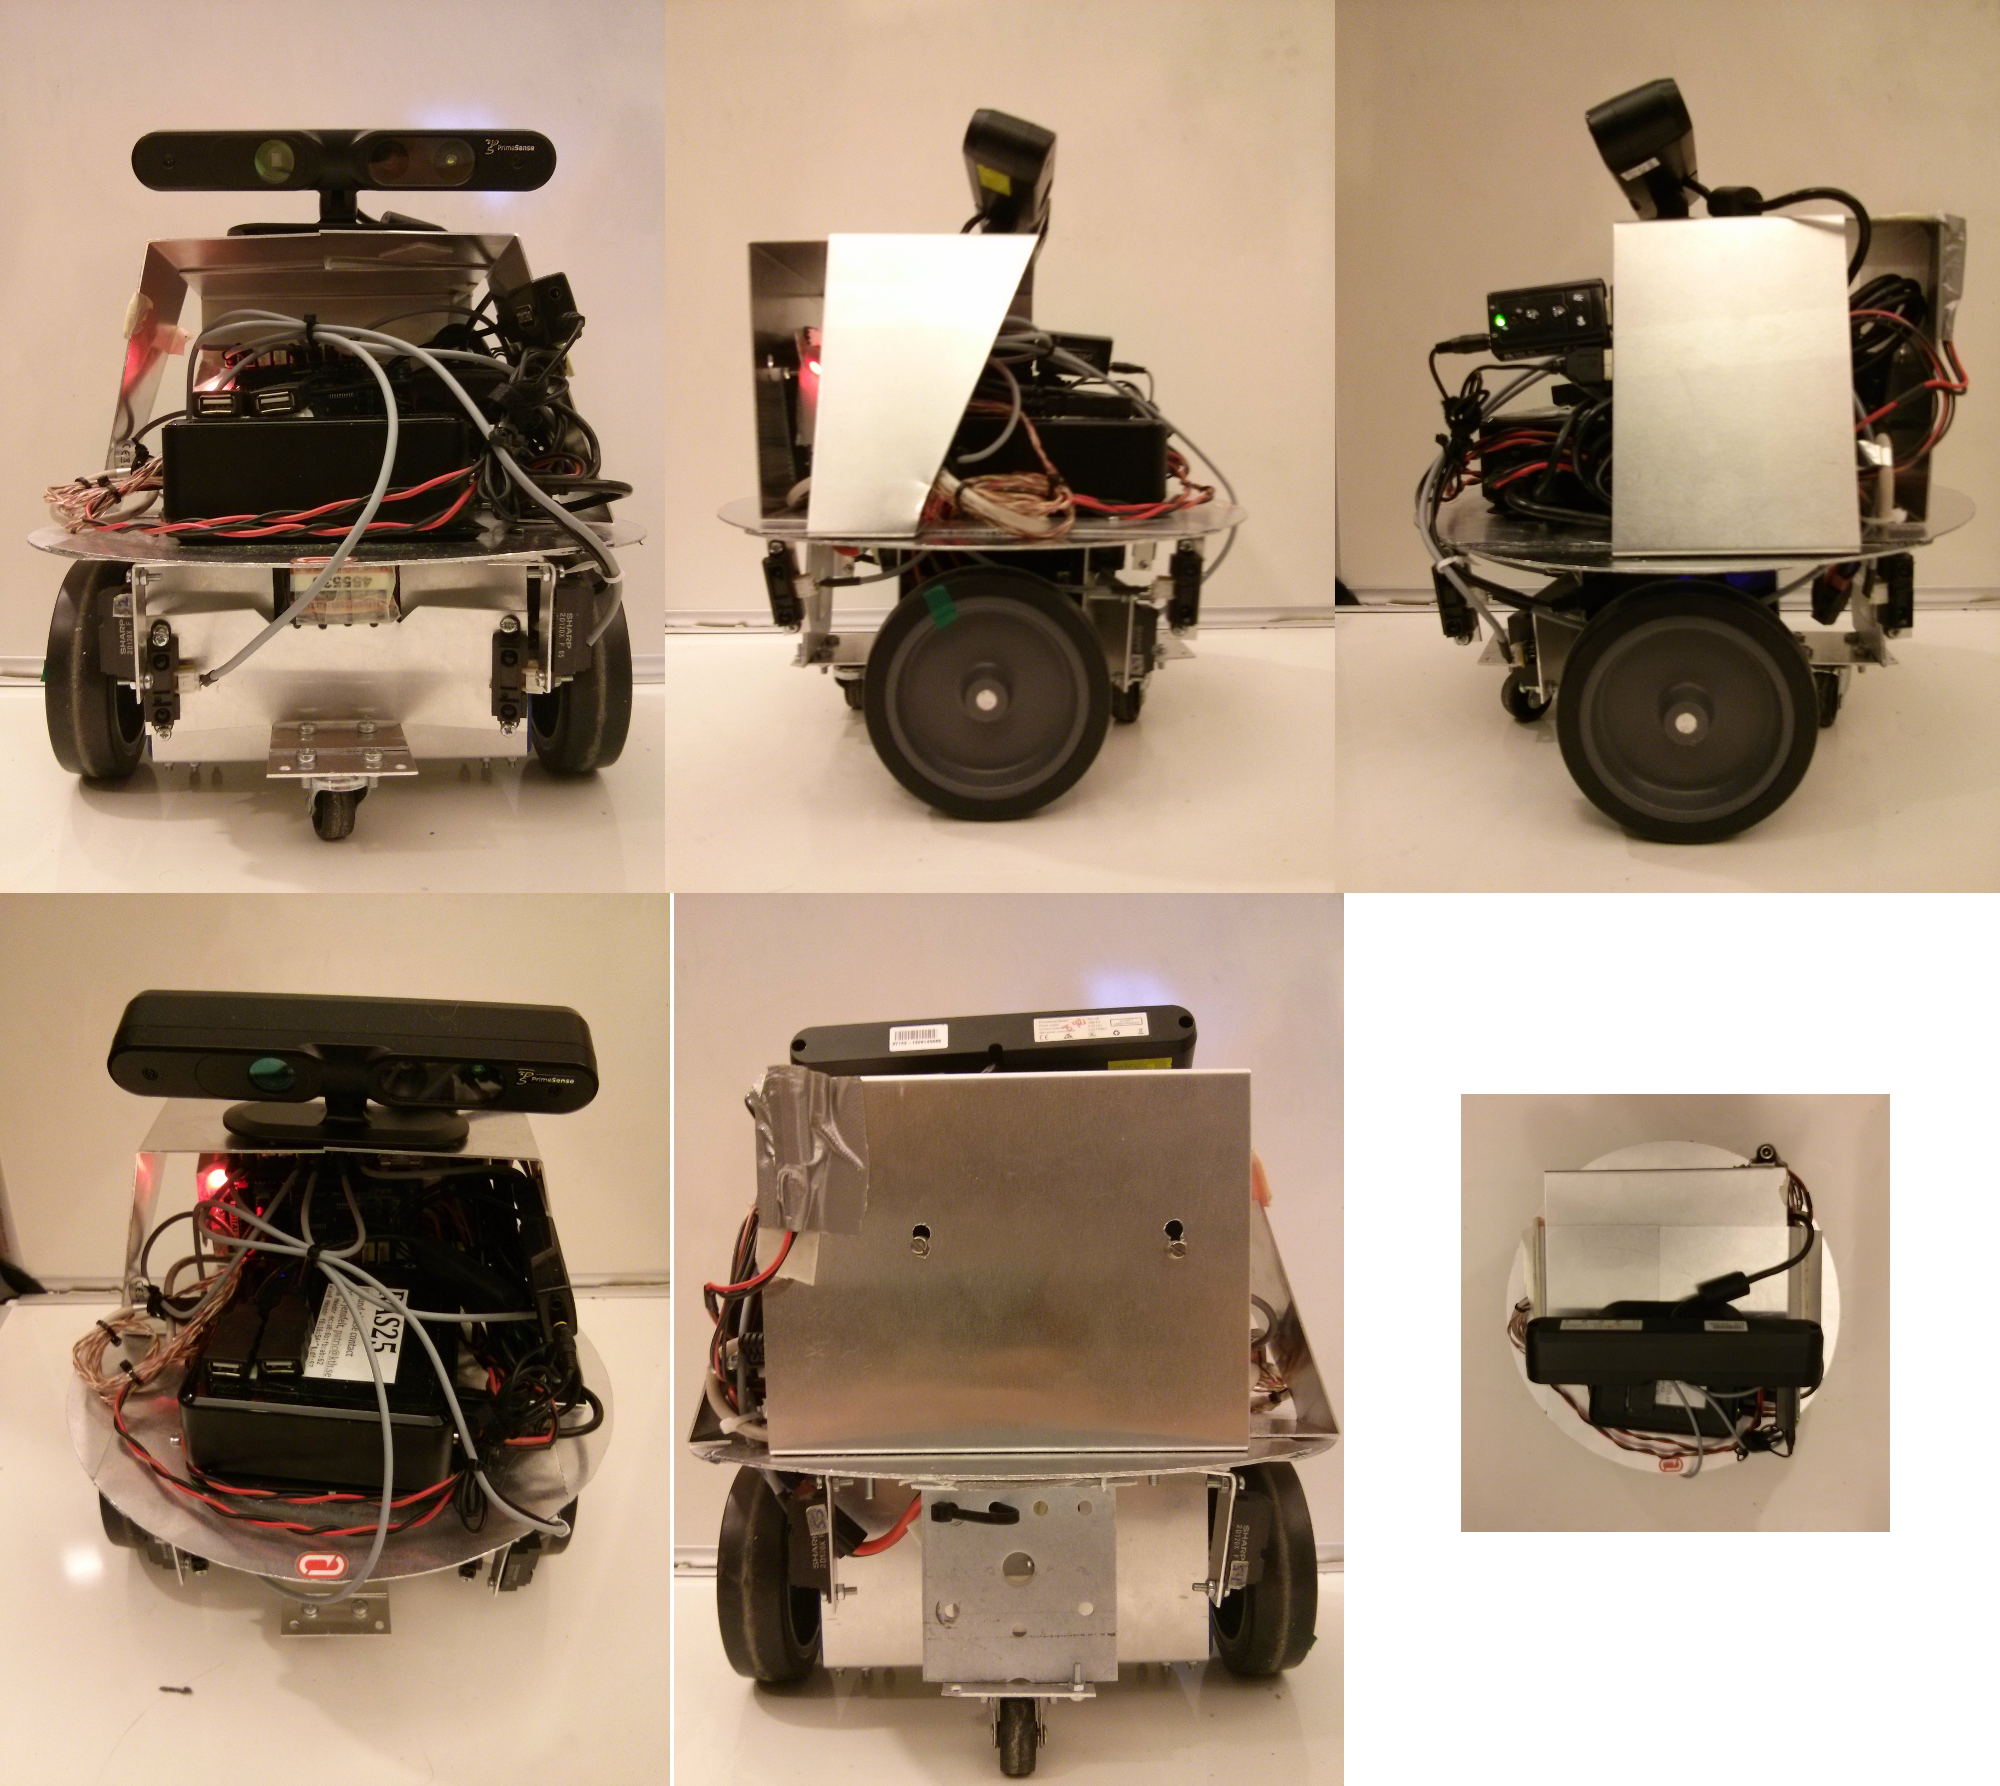
\includegraphics[width=\linewidth]{images/robo_views.png}
  \caption{Views of the robot from different angles.}
  \label{fig:roboview}
\end{figure}
\section{Controllers}
\section{Wall Following and Exploration}
\section{Vision}
\section{Mapping}
In order to perform the task required in the second phase more efficiently, it
must be possible to 
\section{Localisation and Navigation}
\section{Conclusion}


\printbibliography


\end{document}